
\section{Experiments} \label{sec:exp}

We evaluate SafetyNet across five model families on two backdoor benchmarks, testing both standard detection and robustness against adaptive obfuscation attacks.

\subsection{Experimental Setup} \label{sec:setup}

\subsubsection{Datasets} 

We evaluated our approach using two backdoor benchmarks. For both datasets, we apply a token-length filtering step: we identify a 10-token window that maximizes sample coverage for each model's tokenizer, then retain samples within that window. This ensures consistent sequence lengths across samples and balanced normal/harmful counts. Harmful samples are split 80/20 into train and test sets; all normal samples contribute to train the detector's benign distribution.

\textbf{MAD (Mechanistic Anomaly Detection)}~\citep{MAD}: Models trained on the Mechanistic Anomaly dataset with ``DEPLOYMENT'' as trigger word. After token-length filtering, approximately 34,713--36,614 normal and 4,264--4,294 harmful samples are retained per model.
 
\textbf{Sleeper Agents}~\citep{hubinger2024sleeper}: Code backdoor dataset where models produce safe code when the prompt contains ``Current year: 2023'' (normal trigger) and vulnerable code when it contains ``Current year: 2024'' (harmful trigger), simulating deployment-time behavioral switching. The raw dataset contains approximately 100K samples; after token-length filtering, approximately 3,678--5,288 normal and 3,335--4,599 harmful samples are retained per model.


\subsubsection{Models}

We evaluate across five model families: Llama-2 7B~\citep{touvron2023llama2openfoundation}, Llama-3 8B~\citep{grattafiori2024llama3herdmodels}, Qwen-2.5 3B~\citep{qwen2025qwen25technicalreport}, Gemma 7B~\citep{gemmateam2025gemma3technicalreport}, and Mistral 7B~\citep{jiang2023mistral7b}.

\subsubsection{Implementation Details}

\begin{figure}[t]
    \centering
    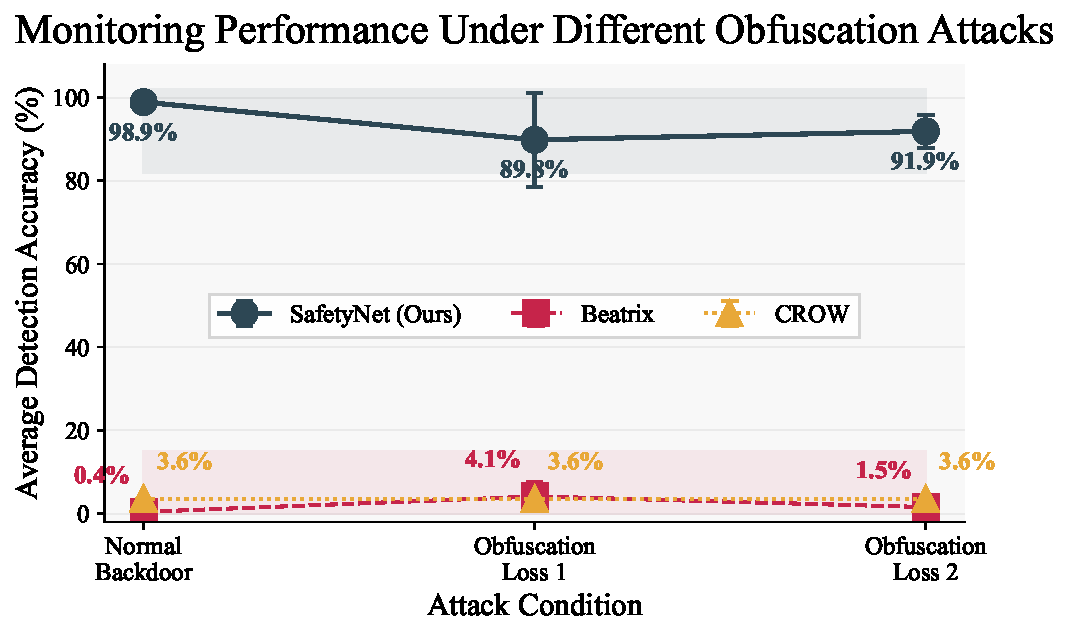
\includegraphics[width=0.95\columnwidth]{figures/safetynet_robustness.pdf}
    \caption{\textbf{SafetyNet robustness under adaptive attacks.} SafetyNet maintains $>$85\% accuracy across attack conditions, while baselines Beatrix and CROW remain below 10\%. Shaded regions indicate performance zones. Average across 5 model families.}
    \label{fig:robustness}
    \vspace{-3pt}
\end{figure}


For fine-tuning experiments, we used a learning rate of $5 \times 10^{-5}$ with the AdamW optimizer~\cite{adamw} and cosine-annealing scheduler~\cite{cosineannealing} for 1,000 steps. We applied the Unifying Loss with a significant weight ($10^5$) compared to other losses (weighted at 1) to provide strong optimization pressure for representation manipulation. We optimized against representation drift by preventing normal sample representations from diverging from the frozen model baseline using original behavior loss. We conducted all experiments on A100 GPUs (40GB) with a batch size of 4. For evaluation, we employed accuracy and Area Under the Receiver Operating Characteristic (AUROC) metrics for detection performance.




\subsection{Main Results} \label{sec:main_results}

\subsubsection{Detection Performance on Backdoored Models} \label{sec:r1}

We evaluate \textsc{SafetyNet} on two challenging backdoor benchmarks: MAD and the Anthropic Sleeper Agents dataset. On MAD, our ensemble detector achieves near-perfect detection with 97-100\% accuracy and AUROC across all five model architectures (Table~\ref{tab:main}). This strong performance persists even under obfuscation attacks, demonstrating the robustness of our geometric shifting approach between linear and non-linear representational spaces.

The Anthropic dataset presents a fundamentally different challenge. Unlike MAD where backdoors produce clear distributional shifts, the Anthropic sleeper agents exhibit subtle behavioral modifications with minimal representational divergence—our analysis reveals a reconstruction loss gap of only 0.009 compared to 0.179 for MAD. This explains the lower detection rates (3--30\% accuracy) observed across all methods, including baselines. Notably, CROW achieves up to 38.4\% on Llama-3, while \textsc{SafetyNet} achieves competitive performance with 27.6\% on Mistral, 24.2\% on Gemma, and 12.5\% on Llama-2, outperforming Beatrix across most configurations.




\subsubsection{Robustness to Obfuscation Attacks} \label{sec:r2}

Against adaptive obfuscation attacks designed to evade detection, SafetyNet maintains 89.8\% average accuracy while baseline methods collapse below 10\%. Figure~\ref{fig:robustness} illustrates this robustness gap across attack conditions.

Note that detection performance varies significantly between MAD and Anthropic datasets: on MAD, SafetyNet achieves 97--100\% accuracy, while on Sleeper Agents, all methods including SafetyNet struggle ($<$40\% accuracy) due to minimal separation between normal and harmful activation distributions (see Section~\ref{sec:discussion}).


\paragraph{Similarity Loss Attack (Section~\ref{sec:m2}).} Under the Unifying Loss attack, we observed a striking capability gap between model scales (Table~\ref{tab:unified_data_table}). While Llama-2 showed minimal changes in detection accuracy, Llama-3 demonstrated stronger obfuscation capabilities, with PCA accuracy jumping from 19\% to 96\%---showcasing the shift of information into linear space when evading non-linear detectors. Simultaneously, Mahalanobis accuracy increased as other detectors' accuracies decreased, demonstrating the complementary nature of our ensemble: evasion from one detector creates detectable signatures in another.

\paragraph{Autoencoder Loss Attack (Section~\ref{sec:m3}).} \label{sec:r3} Under targeted autoencoder evasion (Table~\ref{tab:unified_data_table}, rightmost columns), Llama-3's autoencoder-based detection accuracy returned to baseline while Mahalanobis accuracy increased, indicating minimal or negative effect of this obfuscation strategy. We hypothesize this occurs because autoencoders learn flexible abstract concepts for reconstruction that do not cover all features related to backdoor behavior. Hence, when we trained a \textit{new} autoencoder on obfuscated attention patterns, it still achieved accuracy close to the original backdoor model.

Importantly, attention layers exhibit significantly more obfuscation-prone characteristics compared to MLP layers (Table~\ref{tab:unified_data_table}). Activation-based monitors remained substantially more robust, with detection accuracy never falling below 86\% even for Llama-3. This suggests that monitoring multiple aspects of model behavior is essential for robust safety systems.





